\documentclass[border=2pt]{standalone}
\usepackage{tikz}
\usetikzlibrary{arrows.meta,chains}

\begin{document}
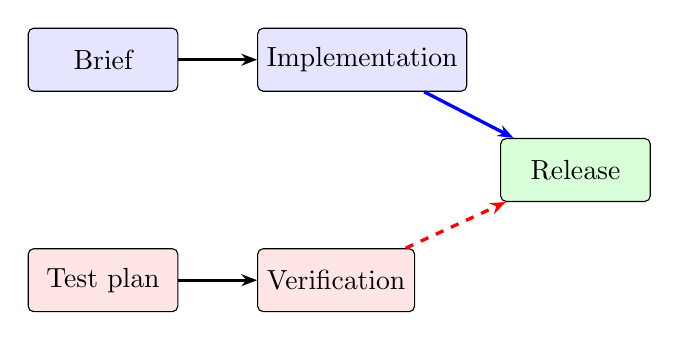
\begin{tikzpicture}[
  node distance=5mm and 10mm,
  start chain=design going right,
  start chain=quality going right,
  start chain=delivery going right,
  stage/.style={draw,rounded corners=2pt,minimum width=19mm,minimum height=8mm,align=center},
  every on chain/.style={join},
  every join/.style={-{Stealth[length=2mm]},very thick}
]
  \node[stage,on chain=design,fill=blue!10] (brief) at (0,1.4) {Brief};
  \node[stage,on chain=design,fill=blue!10] (implementation) {Implementation};

  \node[stage,on chain=quality,fill=red!10] (test-plan) at (0,-1.4) {Test plan};
  \node[stage,on chain=quality,fill=red!10] (verification) {Verification};

  \node[
    stage,
    on chain=delivery,
    fill=green!15,
    join=with design-end by {blue},
    join=with quality-end by {red,dashed}
  ] (release) at (6,0) {Release};
\end{tikzpicture}
\end{document}
